
\section{DNS}

\subsection{Скриншоты}

\begin{center}

    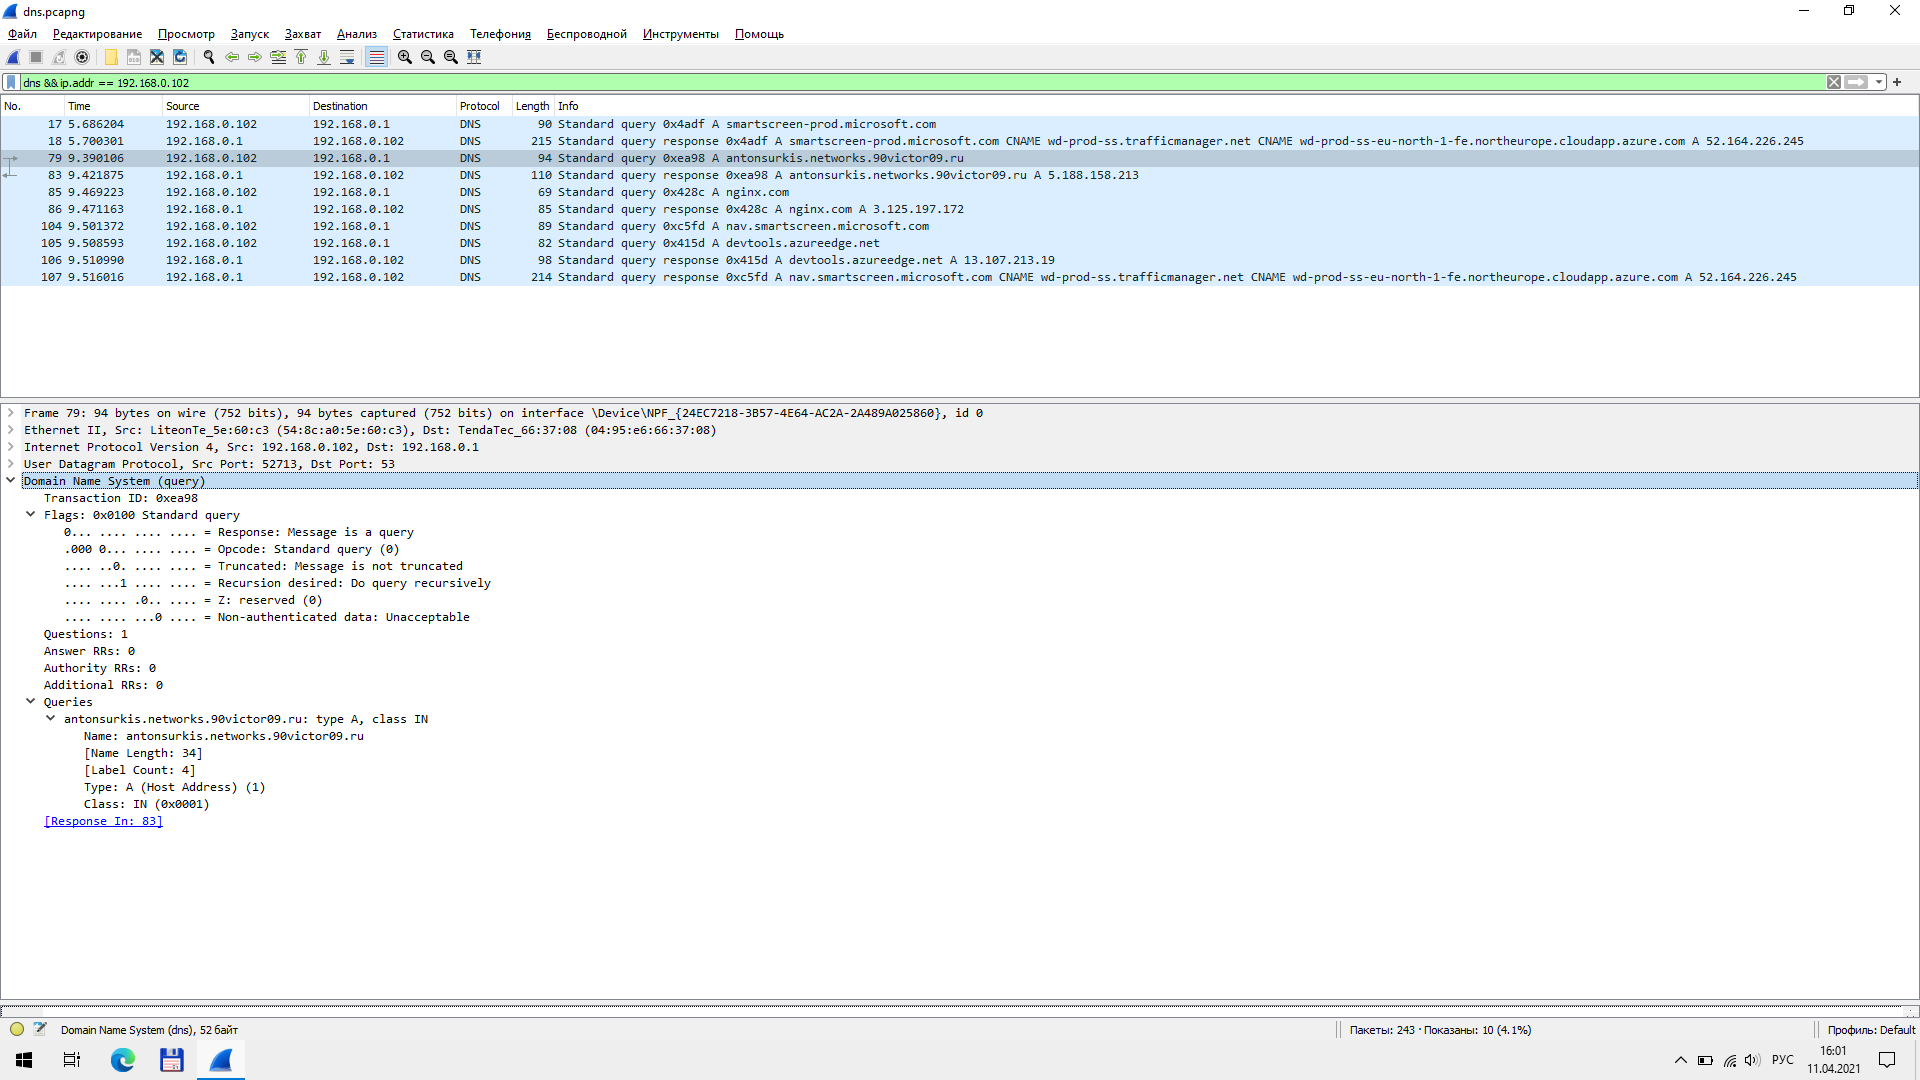
\includegraphics[width=\textwidth]{screenshots/dns_request_1}

    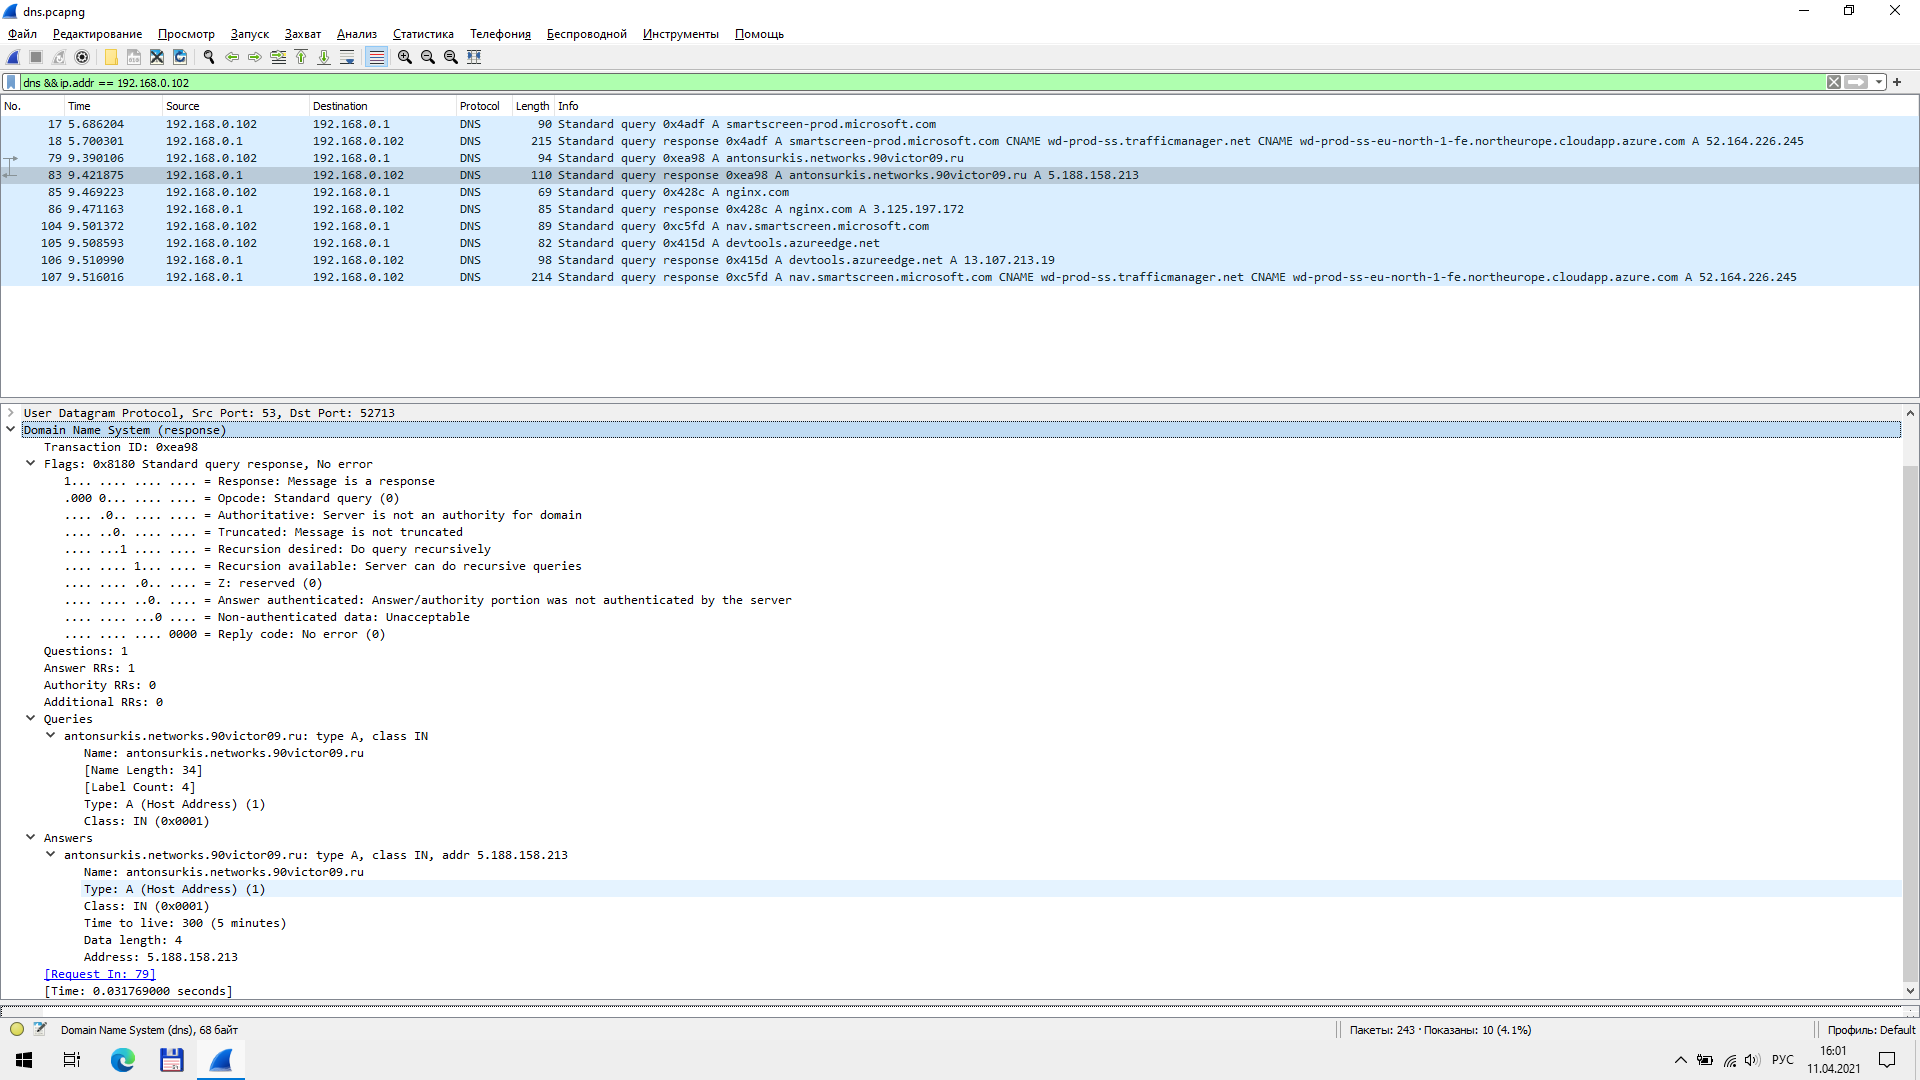
\includegraphics[width=\textwidth]{screenshots/dns_response_1}

\end{center}

\subsection{Ответы на вопросы}

\subsubsection{}
Потому что DNS-запрос производится в локальной сети --- к контроллерам, к которым у компьютера есть физический доступ.

\subsubsection{}
\begin{enumerate}
    \item Рекурсивные --- поиск по кусочкам домена, начиная от верхнего уровня (ru, com, net, \ldots);
    \item Итеративные --- обмен записями кеша между DNS-серверами;
    \item Инверсные --- при известном IP запрашивается доменное имя.
\end{enumerate}

\subsubsection{}
Если изображения находятся на другом домене или если домен сайта разрешается в разные адреса (например,
как в случае с YouTube или Discord).
